% Options for packages loaded elsewhere
\PassOptionsToPackage{unicode}{hyperref}
\PassOptionsToPackage{hyphens}{url}
%
\documentclass[
]{article}
\usepackage{amsmath,amssymb}
\usepackage{iftex}
\ifPDFTeX
  \usepackage[T1]{fontenc}
  \usepackage[utf8]{inputenc}
  \usepackage{textcomp} % provide euro and other symbols
\else % if luatex or xetex
  \usepackage{unicode-math} % this also loads fontspec
  \defaultfontfeatures{Scale=MatchLowercase}
  \defaultfontfeatures[\rmfamily]{Ligatures=TeX,Scale=1}
\fi
\usepackage{lmodern}
\ifPDFTeX\else
  % xetex/luatex font selection
\fi
% Use upquote if available, for straight quotes in verbatim environments
\IfFileExists{upquote.sty}{\usepackage{upquote}}{}
\IfFileExists{microtype.sty}{% use microtype if available
  \usepackage[]{microtype}
  \UseMicrotypeSet[protrusion]{basicmath} % disable protrusion for tt fonts
}{}
\makeatletter
\@ifundefined{KOMAClassName}{% if non-KOMA class
  \IfFileExists{parskip.sty}{%
    \usepackage{parskip}
  }{% else
    \setlength{\parindent}{0pt}
    \setlength{\parskip}{6pt plus 2pt minus 1pt}}
}{% if KOMA class
  \KOMAoptions{parskip=half}}
\makeatother
\usepackage{xcolor}
\usepackage[margin=1in]{geometry}
\usepackage{color}
\usepackage{fancyvrb}
\newcommand{\VerbBar}{|}
\newcommand{\VERB}{\Verb[commandchars=\\\{\}]}
\DefineVerbatimEnvironment{Highlighting}{Verbatim}{commandchars=\\\{\}}
% Add ',fontsize=\small' for more characters per line
\usepackage{framed}
\definecolor{shadecolor}{RGB}{248,248,248}
\newenvironment{Shaded}{\begin{snugshade}}{\end{snugshade}}
\newcommand{\AlertTok}[1]{\textcolor[rgb]{0.94,0.16,0.16}{#1}}
\newcommand{\AnnotationTok}[1]{\textcolor[rgb]{0.56,0.35,0.01}{\textbf{\textit{#1}}}}
\newcommand{\AttributeTok}[1]{\textcolor[rgb]{0.13,0.29,0.53}{#1}}
\newcommand{\BaseNTok}[1]{\textcolor[rgb]{0.00,0.00,0.81}{#1}}
\newcommand{\BuiltInTok}[1]{#1}
\newcommand{\CharTok}[1]{\textcolor[rgb]{0.31,0.60,0.02}{#1}}
\newcommand{\CommentTok}[1]{\textcolor[rgb]{0.56,0.35,0.01}{\textit{#1}}}
\newcommand{\CommentVarTok}[1]{\textcolor[rgb]{0.56,0.35,0.01}{\textbf{\textit{#1}}}}
\newcommand{\ConstantTok}[1]{\textcolor[rgb]{0.56,0.35,0.01}{#1}}
\newcommand{\ControlFlowTok}[1]{\textcolor[rgb]{0.13,0.29,0.53}{\textbf{#1}}}
\newcommand{\DataTypeTok}[1]{\textcolor[rgb]{0.13,0.29,0.53}{#1}}
\newcommand{\DecValTok}[1]{\textcolor[rgb]{0.00,0.00,0.81}{#1}}
\newcommand{\DocumentationTok}[1]{\textcolor[rgb]{0.56,0.35,0.01}{\textbf{\textit{#1}}}}
\newcommand{\ErrorTok}[1]{\textcolor[rgb]{0.64,0.00,0.00}{\textbf{#1}}}
\newcommand{\ExtensionTok}[1]{#1}
\newcommand{\FloatTok}[1]{\textcolor[rgb]{0.00,0.00,0.81}{#1}}
\newcommand{\FunctionTok}[1]{\textcolor[rgb]{0.13,0.29,0.53}{\textbf{#1}}}
\newcommand{\ImportTok}[1]{#1}
\newcommand{\InformationTok}[1]{\textcolor[rgb]{0.56,0.35,0.01}{\textbf{\textit{#1}}}}
\newcommand{\KeywordTok}[1]{\textcolor[rgb]{0.13,0.29,0.53}{\textbf{#1}}}
\newcommand{\NormalTok}[1]{#1}
\newcommand{\OperatorTok}[1]{\textcolor[rgb]{0.81,0.36,0.00}{\textbf{#1}}}
\newcommand{\OtherTok}[1]{\textcolor[rgb]{0.56,0.35,0.01}{#1}}
\newcommand{\PreprocessorTok}[1]{\textcolor[rgb]{0.56,0.35,0.01}{\textit{#1}}}
\newcommand{\RegionMarkerTok}[1]{#1}
\newcommand{\SpecialCharTok}[1]{\textcolor[rgb]{0.81,0.36,0.00}{\textbf{#1}}}
\newcommand{\SpecialStringTok}[1]{\textcolor[rgb]{0.31,0.60,0.02}{#1}}
\newcommand{\StringTok}[1]{\textcolor[rgb]{0.31,0.60,0.02}{#1}}
\newcommand{\VariableTok}[1]{\textcolor[rgb]{0.00,0.00,0.00}{#1}}
\newcommand{\VerbatimStringTok}[1]{\textcolor[rgb]{0.31,0.60,0.02}{#1}}
\newcommand{\WarningTok}[1]{\textcolor[rgb]{0.56,0.35,0.01}{\textbf{\textit{#1}}}}
\usepackage{graphicx}
\makeatletter
\def\maxwidth{\ifdim\Gin@nat@width>\linewidth\linewidth\else\Gin@nat@width\fi}
\def\maxheight{\ifdim\Gin@nat@height>\textheight\textheight\else\Gin@nat@height\fi}
\makeatother
% Scale images if necessary, so that they will not overflow the page
% margins by default, and it is still possible to overwrite the defaults
% using explicit options in \includegraphics[width, height, ...]{}
\setkeys{Gin}{width=\maxwidth,height=\maxheight,keepaspectratio}
% Set default figure placement to htbp
\makeatletter
\def\fps@figure{htbp}
\makeatother
\setlength{\emergencystretch}{3em} % prevent overfull lines
\providecommand{\tightlist}{%
  \setlength{\itemsep}{0pt}\setlength{\parskip}{0pt}}
\setcounter{secnumdepth}{-\maxdimen} % remove section numbering
\ifLuaTeX
  \usepackage{selnolig}  % disable illegal ligatures
\fi
\usepackage{bookmark}
\IfFileExists{xurl.sty}{\usepackage{xurl}}{} % add URL line breaks if available
\urlstyle{same}
\hypersetup{
  pdftitle={Forecasting Competition Report},
  pdfauthor={Rachael Stephan \& Rosie Wu},
  hidelinks,
  pdfcreator={LaTeX via pandoc}}

\title{Forecasting Competition Report}
\author{Rachael Stephan \& Rosie Wu}
\date{}

\begin{document}
\maketitle

\href{https://github.com/rachls/StephanWu_ENV797_TSA_ForecastCompetition_S25}{Github
Repository}

\section{Introduction}\label{introduction}

This report contains the final deliverable for the forecasting
competition for ENV 797. The objective of this competition was to
produce the best time series forecast of a daily load using various
models and exogenous factors of humidity and temperature. This report
contains the workings for the 5 top performing models.

\section{Data Source}\label{data-source}

Data was retrieved from the
\href{https://www.kaggle.com/competitions/tsa-spring-2025/data}{Kaggle
competition site}. All data was provided by instructor Luana Lima.

\section{Wrangling}\label{wrangling}

The hourly load data frame were uploaded into R and wrangled as follows
to produced both daily and hourly data.

Daily Data:

\begin{itemize}
\tightlist
\item
  Format date columns as date.
\item
  Aggregate data frame by row with \texttt{rowwise()}
\item
  Calculate the daily load as the mean of every hour.
\item
  Ungroup the data frame from \texttt{rowwise()}
\item
  Drop unnecessary columns (i.e., hourly data and meter id)
\end{itemize}

\begin{Shaded}
\begin{Highlighting}[]
\CommentTok{\#load data and create a daily average data frame}
\NormalTok{dailyload }\OtherTok{\textless{}{-}}\NormalTok{ readxl}\SpecialCharTok{::}\FunctionTok{read\_xlsx}\NormalTok{(}\StringTok{"./Data/Raw/load.xlsx"}\NormalTok{) }\SpecialCharTok{\%\textgreater{}\%}
    \FunctionTok{mutate}\NormalTok{(}\AttributeTok{date =} \FunctionTok{as.Date}\NormalTok{(date, }\AttributeTok{format =} \StringTok{"\%Y{-}\%m{-}\%d"}\NormalTok{)) }\SpecialCharTok{\%\textgreater{}\%}  
    \FunctionTok{rowwise}\NormalTok{() }\SpecialCharTok{\%\textgreater{}\%}
    \FunctionTok{mutate}\NormalTok{(}\AttributeTok{daily\_average =} \FunctionTok{mean}\NormalTok{(}\FunctionTok{c\_across}\NormalTok{(h1}\SpecialCharTok{:}\NormalTok{h24), }\AttributeTok{na.rm =} \ConstantTok{TRUE}\NormalTok{)) }\SpecialCharTok{\%\textgreater{}\%}  
    \FunctionTok{ungroup}\NormalTok{() }\SpecialCharTok{\%\textgreater{}\%}
    \FunctionTok{select}\NormalTok{(}\SpecialCharTok{{-}}\FunctionTok{c}\NormalTok{(h1}\SpecialCharTok{:}\NormalTok{h24), }\SpecialCharTok{{-}}\NormalTok{meter\_id)}
\end{Highlighting}
\end{Shaded}

Hourly Data:

\begin{itemize}
\tightlist
\item
  Format date columns as date.
\item
  Calculate the daily load as the mean of every hour.
\item
  pivot data frame longer to put the hour into one column and the hourly
  load into another.
\item
  Extract hour integer and reformat hour column as integer data.
\item
  Drop unnecessary columns (i.e., meter id)
\end{itemize}

\begin{Shaded}
\begin{Highlighting}[]
\CommentTok{\#load data and create an hourly average data frame}
\NormalTok{hourlyload }\OtherTok{\textless{}{-}}\NormalTok{ readxl}\SpecialCharTok{::}\FunctionTok{read\_xlsx}\NormalTok{(}\StringTok{"./Data/Raw/load.xlsx"}\NormalTok{) }\SpecialCharTok{\%\textgreater{}\%}
    \FunctionTok{mutate}\NormalTok{(}\AttributeTok{date =} \FunctionTok{as.Date}\NormalTok{(date, }\AttributeTok{format =} \StringTok{"\%Y{-}\%m{-}\%d"}\NormalTok{)) }\SpecialCharTok{\%\textgreater{}\%}  
    \FunctionTok{pivot\_longer}\NormalTok{(}\AttributeTok{cols =} \FunctionTok{starts\_with}\NormalTok{(}\StringTok{"h"}\NormalTok{),}
                 \AttributeTok{names\_to =} \StringTok{"hour"}\NormalTok{,}
                 \AttributeTok{values\_to =} \StringTok{"load"}\NormalTok{)}\SpecialCharTok{\%\textgreater{}\%}
    \FunctionTok{mutate}\NormalTok{(}\AttributeTok{hour =} \FunctionTok{as.integer}\NormalTok{(}\FunctionTok{substring}\NormalTok{(hour,}\DecValTok{2}\NormalTok{))) }\SpecialCharTok{\%\textgreater{}\%}
    \FunctionTok{select}\NormalTok{(}\SpecialCharTok{{-}}\NormalTok{meter\_id)}
\end{Highlighting}
\end{Shaded}

\subsection{Section Data}\label{section-data}

Data was wrangled into training (n = 2141) and test (n = 50)
observations. These were used to evaluate our models before uploading to
Kaggle.

\begin{Shaded}
\begin{Highlighting}[]
\NormalTok{dailyload\_train }\OtherTok{\textless{}{-}} \FunctionTok{head}\NormalTok{(dailyload,}
\NormalTok{                        (}\FunctionTok{length}\NormalTok{(dailyload}\SpecialCharTok{$}\NormalTok{daily\_average)}\SpecialCharTok{{-}}\DecValTok{50}\NormalTok{))}

\NormalTok{dailyload\_test }\OtherTok{\textless{}{-}} \FunctionTok{tail}\NormalTok{(dailyload, }\DecValTok{50}\NormalTok{)}
\end{Highlighting}
\end{Shaded}

\section{Forecasting Methods}\label{forecasting-methods}

The top 5 models were as follows:

\begin{enumerate}
\def\labelenumi{\arabic{enumi}.}
\tightlist
\item
  Neural Network Model (Daily dataset, k= 1, 1, 3)
\item
  model 2
\item
  model 3
\item
  model 4
\item
  model 5
\end{enumerate}

Some models were run on the hourly data, which were averaged into daily
loads after forecasting. However, these models had a very long
processing time. Therefore, we were unable to use these models to
forecast for both the full and training data sets. We ran these models
only on the full data set if our computers were able to process them.
Thus, they are not included in our top 5 models in this report but they
are uploaded onto Kaggle.

\subsection{Model 1}\label{model-1}

\begin{Shaded}
\begin{Highlighting}[]
\CommentTok{\# Set max K values to test}
\NormalTok{max\_K1 }\OtherTok{\textless{}{-}} \DecValTok{3}  \CommentTok{\# For weekly seasonality}
\NormalTok{max\_K2 }\OtherTok{\textless{}{-}} \DecValTok{5}  \CommentTok{\# For yearly seasonality}

\NormalTok{results }\OtherTok{\textless{}{-}} \FunctionTok{expand.grid}\NormalTok{(}\AttributeTok{K1 =} \DecValTok{1}\SpecialCharTok{:}\NormalTok{max\_K1, }\AttributeTok{K2 =} \DecValTok{1}\SpecialCharTok{:}\NormalTok{max\_K2)}
\NormalTok{results}\SpecialCharTok{$}\NormalTok{AICc }\OtherTok{\textless{}{-}} \ConstantTok{NA}

\CommentTok{\# Loop over all K1{-}K2 combinations}
\ControlFlowTok{for}\NormalTok{ (i }\ControlFlowTok{in} \DecValTok{1}\SpecialCharTok{:}\FunctionTok{nrow}\NormalTok{(results)) \{}
\NormalTok{  Kvals }\OtherTok{\textless{}{-}} \FunctionTok{c}\NormalTok{(results}\SpecialCharTok{$}\NormalTok{K1[i], results}\SpecialCharTok{$}\NormalTok{K2[i])}
\NormalTok{  xreg }\OtherTok{\textless{}{-}} \FunctionTok{fourier}\NormalTok{(load\_daily\_msts, }\AttributeTok{K =}\NormalTok{ Kvals)}
  
\NormalTok{  fit }\OtherTok{\textless{}{-}} \FunctionTok{auto.arima}\NormalTok{(load\_daily\_msts, }\AttributeTok{xreg =}\NormalTok{ xreg, }\AttributeTok{seasonal =} \ConstantTok{FALSE}\NormalTok{)}
\NormalTok{  results}\SpecialCharTok{$}\NormalTok{AICc[i] }\OtherTok{\textless{}{-}}\NormalTok{ fit}\SpecialCharTok{$}\NormalTok{aicc}
\NormalTok{\}}

\CommentTok{\# Find best K1{-}K2 pair}
\NormalTok{best\_row }\OtherTok{\textless{}{-}}\NormalTok{ results[}\FunctionTok{which.min}\NormalTok{(results}\SpecialCharTok{$}\NormalTok{AICc), ]}
\FunctionTok{cat}\NormalTok{(}\StringTok{"Best K values: K1 ="}\NormalTok{, best\_row}\SpecialCharTok{$}\NormalTok{K1, }\StringTok{", K2 ="}\NormalTok{, best\_row}\SpecialCharTok{$}\NormalTok{K2, }\StringTok{"}\SpecialCharTok{\textbackslash{}n}\StringTok{"}\NormalTok{)}

\CommentTok{\# Training Data Set}
\NormalTok{fit\_nn\_daily\_train }\OtherTok{\textless{}{-}} \FunctionTok{nnetar}\NormalTok{(}\FunctionTok{as.numeric}\NormalTok{(load\_daily\_train\_msts))}

\NormalTok{forecast\_daily\_nn\_train }\OtherTok{\textless{}{-}} \FunctionTok{forecast}\NormalTok{(fit\_nn\_daily\_train, }
                   \AttributeTok{h=}\DecValTok{59}\NormalTok{)}

\FunctionTok{here}\NormalTok{()}
\FunctionTok{getwd}\NormalTok{()}

\CommentTok{\#write into csv}
\FunctionTok{write.csv}\NormalTok{(forecast\_daily\_nn\_train, }
          \AttributeTok{file =} \StringTok{"../Forecasts/Training/nn2.csv"}\NormalTok{,}
          \AttributeTok{row.names =} \ConstantTok{FALSE}\NormalTok{)}

\NormalTok{fit\_nn\_daily }\OtherTok{\textless{}{-}} \FunctionTok{nnetar}\NormalTok{(}\FunctionTok{as.numeric}\NormalTok{(load\_daily\_msts))}

\NormalTok{forecast\_daily\_nn }\OtherTok{\textless{}{-}} \FunctionTok{forecast}\NormalTok{(fit\_nn\_daily, }
                   \AttributeTok{h=}\DecValTok{59}\NormalTok{)}
\FunctionTok{plot}\NormalTok{(forecast\_daily\_nn)}


\FunctionTok{write.csv}\NormalTok{(forecast\_daily\_nn, }
          \AttributeTok{file =} \StringTok{"../Forecasts/Raw/forecast\_daily\_nn2.csv"}\NormalTok{,}
          \AttributeTok{row.names =} \ConstantTok{FALSE}\NormalTok{)}
\end{Highlighting}
\end{Shaded}

\subsection{Model 2}\label{model-2}

\subsection{Model 3}\label{model-3}

\subsection{Model 4}\label{model-4}

\subsection{Model 5}\label{model-5}

\section{Performance Evaluation}\label{performance-evaluation}

\begin{verbatim}
## here() starts at D:/Spring 2025/StephanWu_ENV797_TSA_ForecastCompetition_S25
\end{verbatim}

\begin{verbatim}
## [1] "D:/Spring 2025/StephanWu_ENV797_TSA_ForecastCompetition_S25"
\end{verbatim}

\begin{verbatim}
## [1] "D:/Spring 2025/StephanWu_ENV797_TSA_ForecastCompetition_S25/Code"
\end{verbatim}

\begin{figure}
\centering
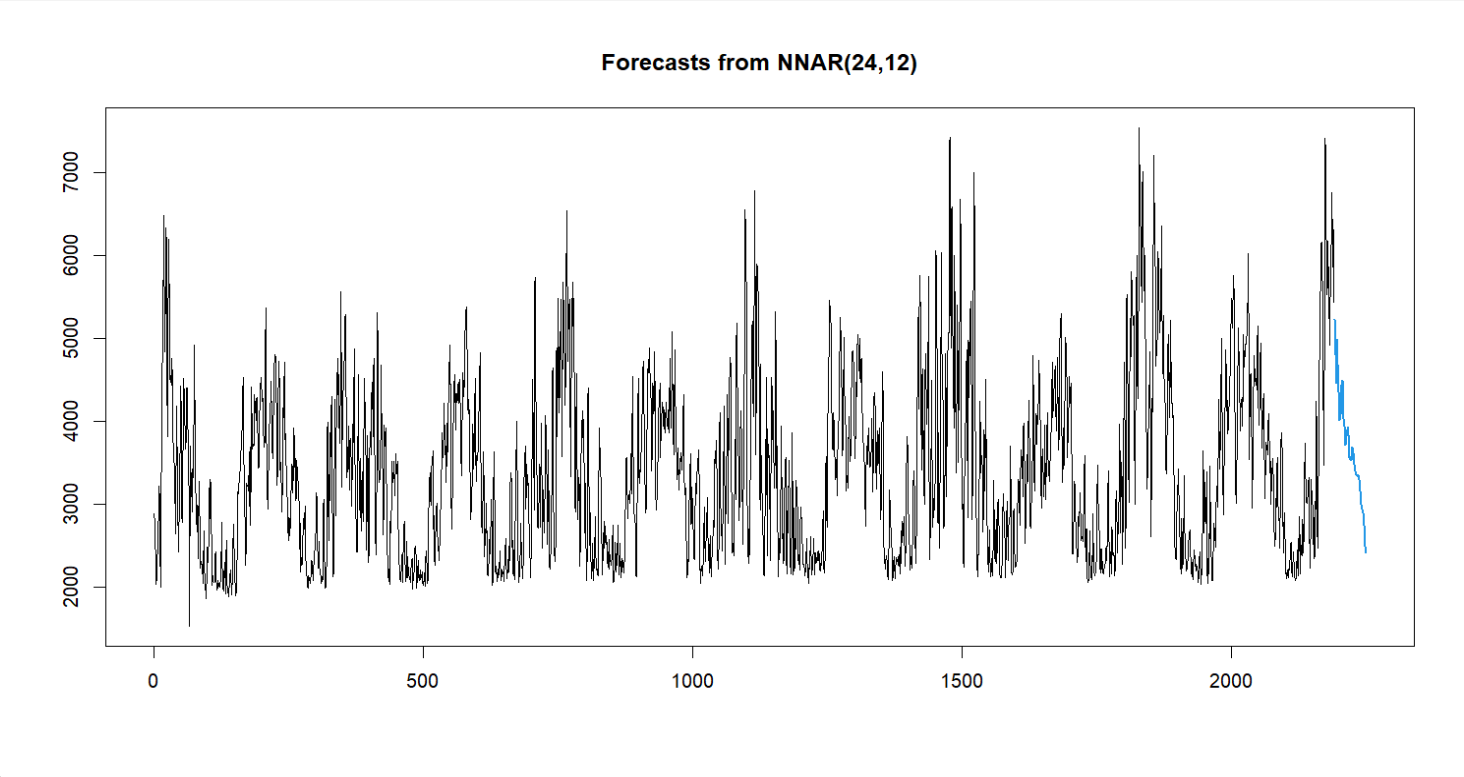
\includegraphics{./Forecasts/NN_daily_113.png}
\caption{NN Daily Forecast}
\end{figure}

include a graph of all 5 forecasts and the performance evaluation table.

\section{Conclusions}\label{conclusions}

A short paragraph about which were the best models, how well they
aligned with

\end{document}
